\documentclass{article}
\usepackage[UTF8]{ctex}
\usepackage{graphicx}
\usepackage{tikz}
\usepackage{eso-pic}
\usepackage{caption}

\AddToShipoutPicture{
	\AtPageLowerLeft{
		\begin{tikzpicture}[remember picture,overlay]
			\node[opacity=0.25,inner sep=0pt] at (current page.center)
			{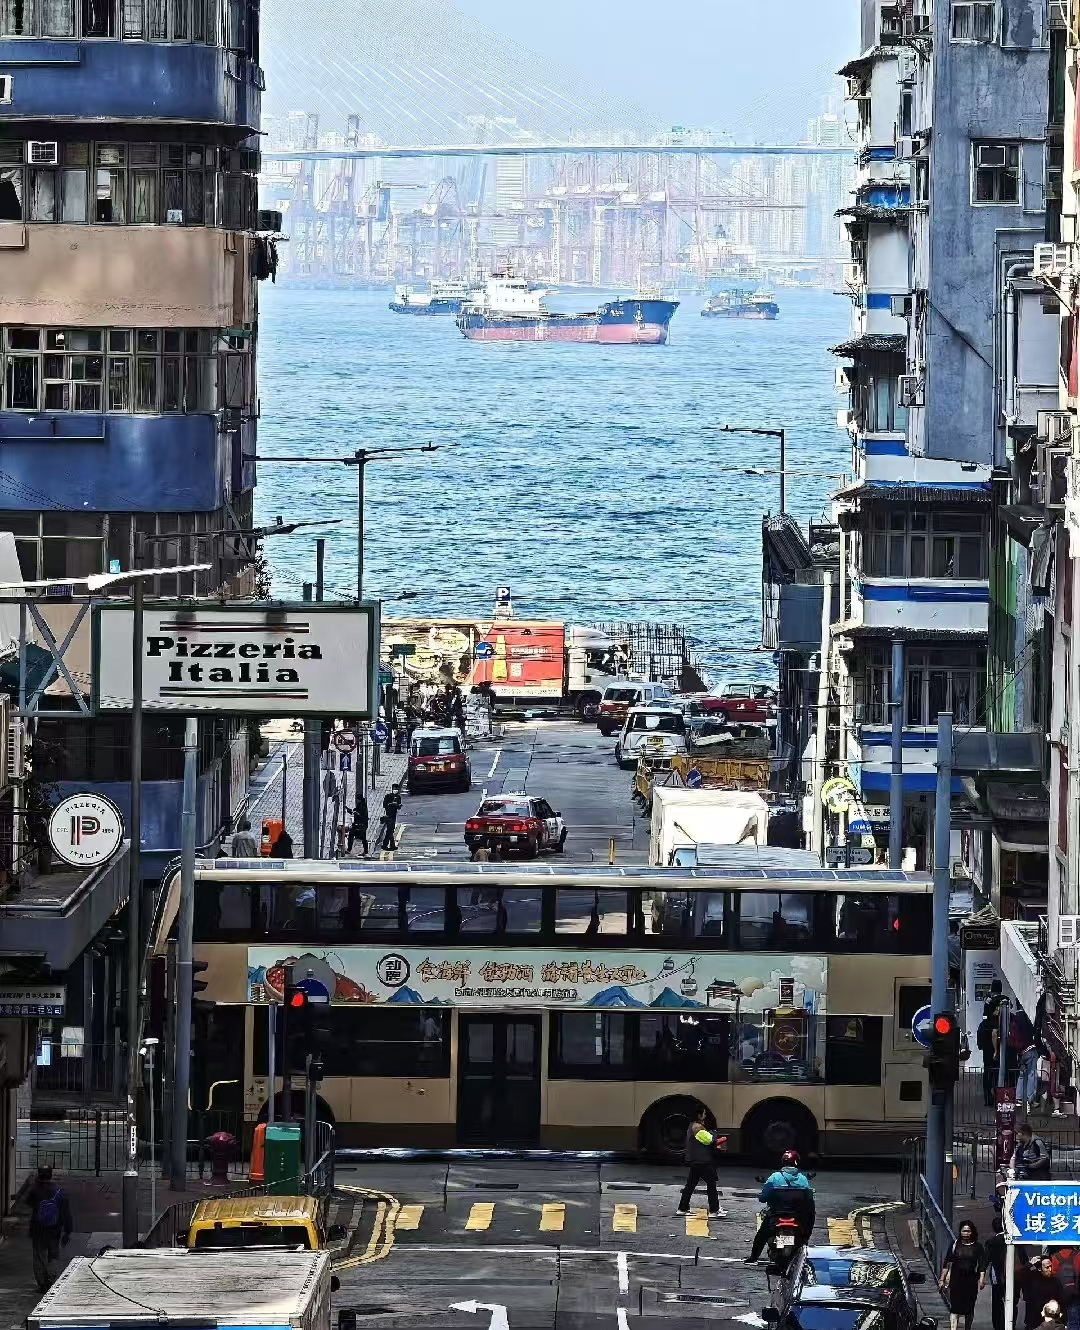
\includegraphics[width=\paperwidth,height=\paperheight]{bk.jpg}};
		\end{tikzpicture}
	}
}

\begin{document}
	\title{\textbf{系统开发工具基础实验报告1}}
	\author{\textbf{程鹏炜}}
	\date{\textbf{2025.8.29}}
	\maketitle
	
	\pagenumbering{Roman}
	\tableofcontents
	\newpage
	\pagenumbering{arabic}
	
	\section{基本实验内容介绍}
	本次实验主要是熟悉相关工具使用和操作实例提高熟练度,主要是latex的相关内容的学习和git工具的使用,latex之前没有接触过但是一上手感觉和html很像,很符合我们计算机玩家把可视化的工具变成命令行的操作,偏向linux的风格。
	
	本次实验由于操作性较少,感觉就像是第一次使用word一样,所有很多流程没有截图使用,尤其是texlive和texstudio的下载过程忘记截图了,额写报告的时候才想起来。
	
	主要是命令行的写法导致不如可视化界面方便我想做的操作需要查询对应的命令是什么。但是写这个感觉还是很不错的像html那样边写边预览,是一个从整体布局到细致分支的感觉。
	
	对于git相关知识,说实话版本控制真没用过,但是git和github相关的命令用过,也老早下过git bash和mingw,后续配置过程就在报告里略去了,
	
	最后是这个实例报告,我就做一个简单的罗列和结果报告。
	
	(逆天latex一段写太多还要overfull警告)
	\newpage
	\section{latex相关工具使用和配置}
	\subsection{配置与安装}
	\begin{figure}[h]  
		\centering
		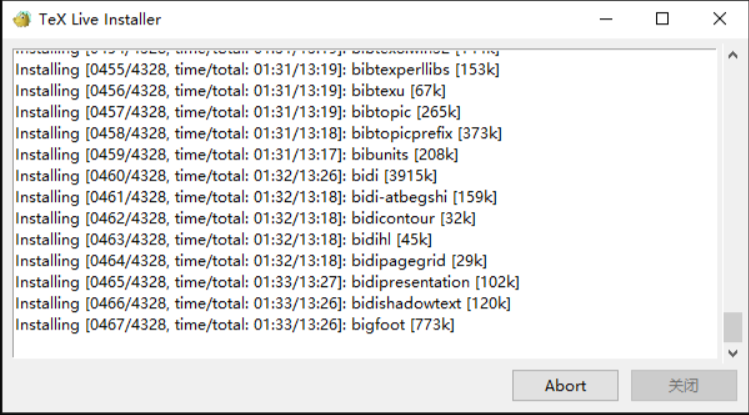
\includegraphics[width=1\textwidth]{a.png}
		\caption{texlive安装}
		\label{fig:example1}
	\end{figure}

	texlive的安装过程,见图\ref{fig:example1}
	
	本来是直接下载本地的但是太慢了还是下载了清华镜像源,然后选ios文件这样最快,在浏览器里面可以使用idm多线程下载,完成后直接挂载ios文件,离线安装就好了,但是总共还是用了好几个小时。
	
	\begin{figure}[h]  
		\centering
		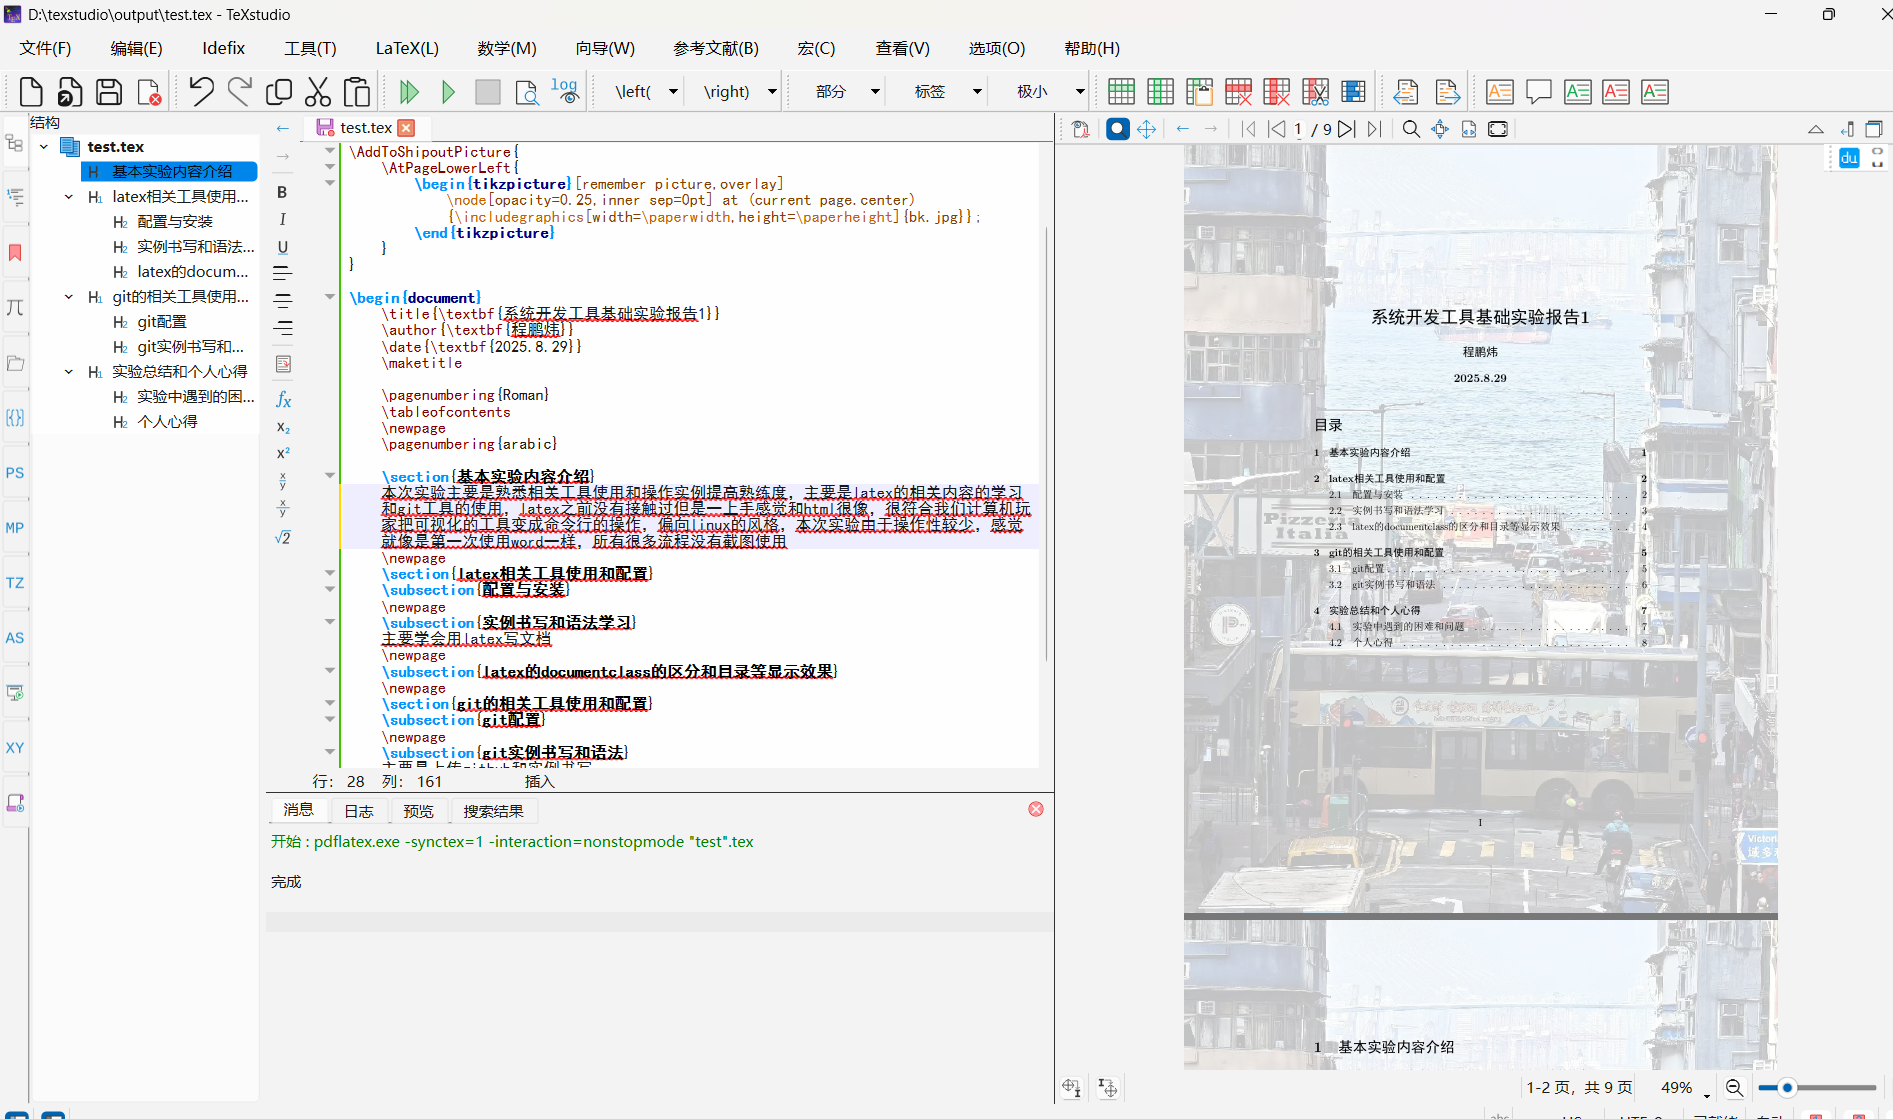
\includegraphics[width=1\textwidth]{b.png}
		\caption{textstudio配置使用}
		\label{fig:example2}
	\end{figure}
	
	texlive下载下来只能作为一个编译环境,见图\ref{fig:example2}
	
	我下载一个textstudio作为编译器,当然我们可以使用vscode但是嘞还要下插件配置很多东西,肯定没有专业的textstufio方便,下载完之后,只要texlive添加到环境变量后,内部配置选好编译环境就可以了。
	
	以上是关于latex书写的环境和工具的安装和配置,一些上手基础在overleaf网页版进行过简单的操作,包括创建标题,创建目录,设置字体插入图表等等。
	
	\newpage
	
	\subsection{实例书写和语法学习}
	主要学会用latex写文档
	
	实例列举:
	
	1.使用documentclass配合begin end创建文章,主要有article report book这些类型。见图\ref{fig:example3}
	
	\begin{figure}[h]  
		\centering
		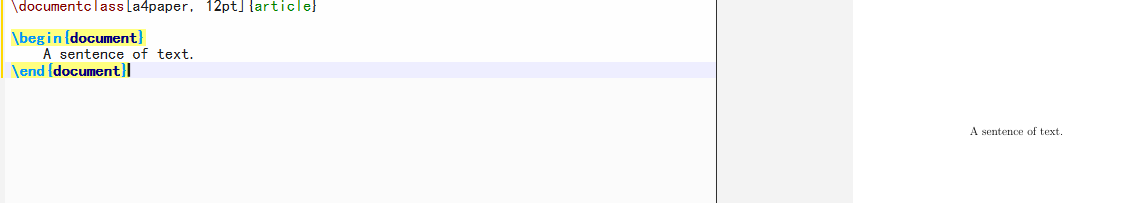
\includegraphics[width=1\textwidth]{d.png}
		\caption{实例1:创建article}
		\label{fig:example3}
	\end{figure}
	
	\newpage
	
	2.使用title,maketitle指令创建标题。见图\ref{fig:example4}
	
	\begin{figure}[h]  
		\centering
		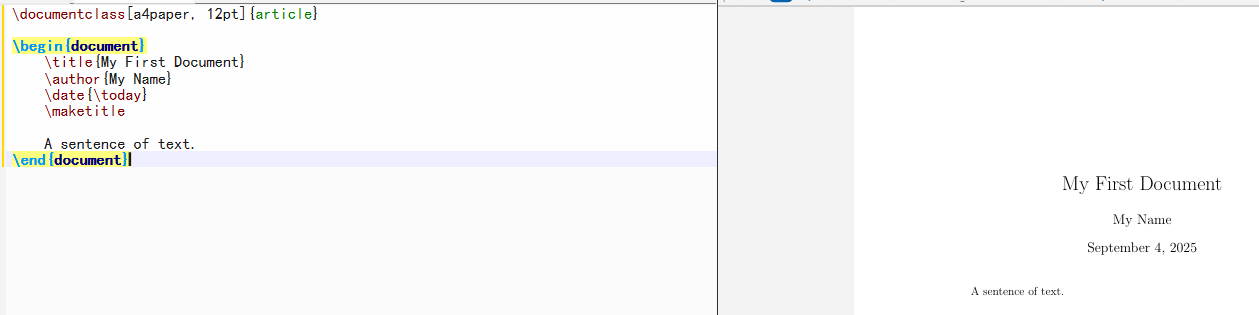
\includegraphics[width=1\textwidth]{e.png}
		\caption{实例2:创建title}
		\label{fig:example4}
	\end{figure}
	
	3.使用sectiion指令创建小标题。见图\ref{fig:example5}
	
	\begin{figure}[h]  
		\centering
		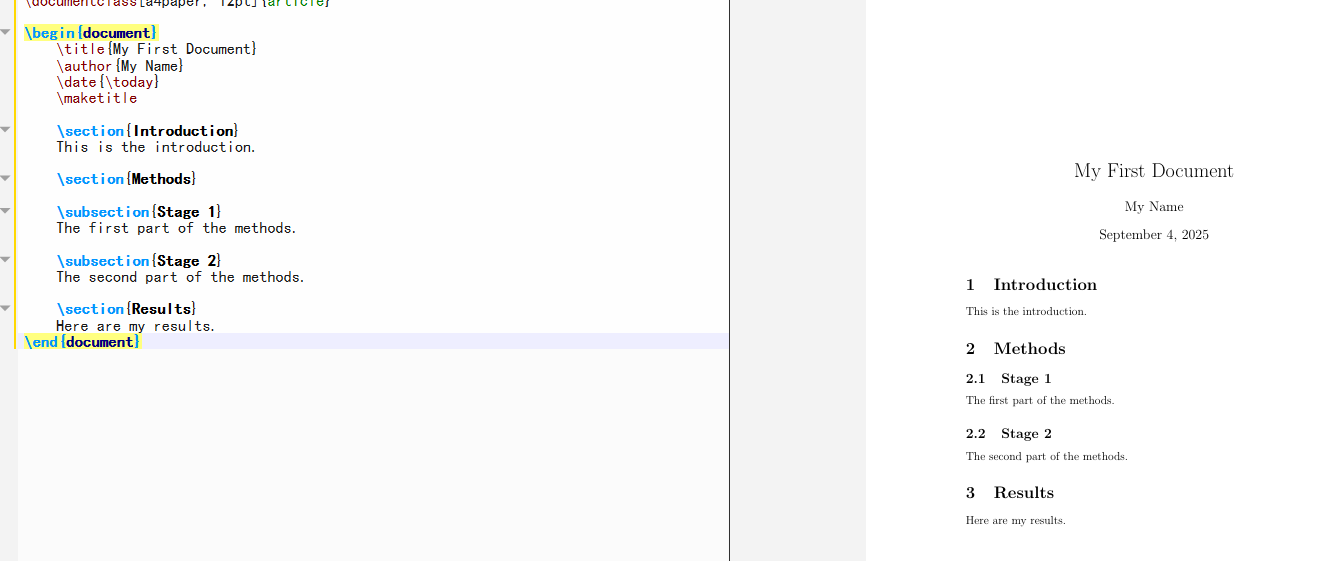
\includegraphics[width=1\textwidth]{f.png}
		\caption{实例3:section创建章节}
		\label{fig:example5}
	\end{figure}
	
	4.使用tableofcontents创建目录。见图\ref{fig:example6}
	
	\begin{figure}[h]  
		\centering
		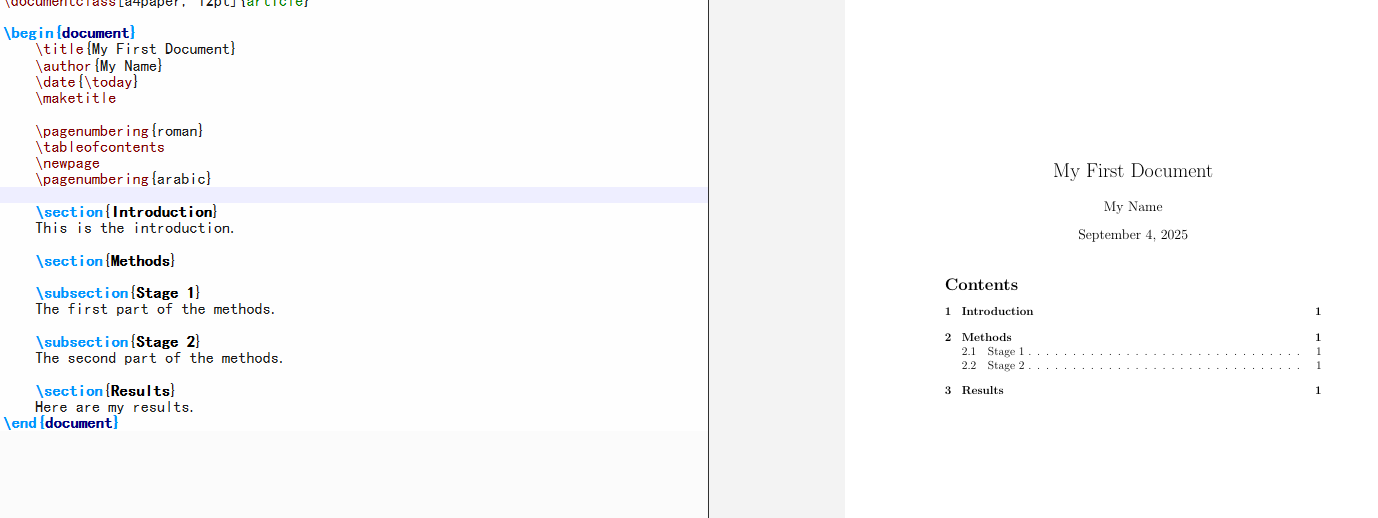
\includegraphics[width=1\textwidth]{g.png}
		\caption{实例4:创建目录}
		\label{fig:example6}
	\end{figure}
	
	\newpage
	
	5.使用pagenumbering设置页码格式:roman小写罗马字体,Roman大写,阿拉伯。见图\ref{fig:example7}
	
	\begin{figure}[h]  
		\centering
		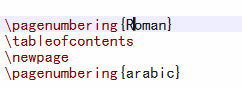
\includegraphics[width=1\textwidth]{h.png}
		\caption{实例5:页码设置}
		\label{fig:example7}
	\end{figure}
	
	6.使用textbf设置粗体。见图\ref{fig:example8}
	
	\begin{figure}[h]  
		\centering
		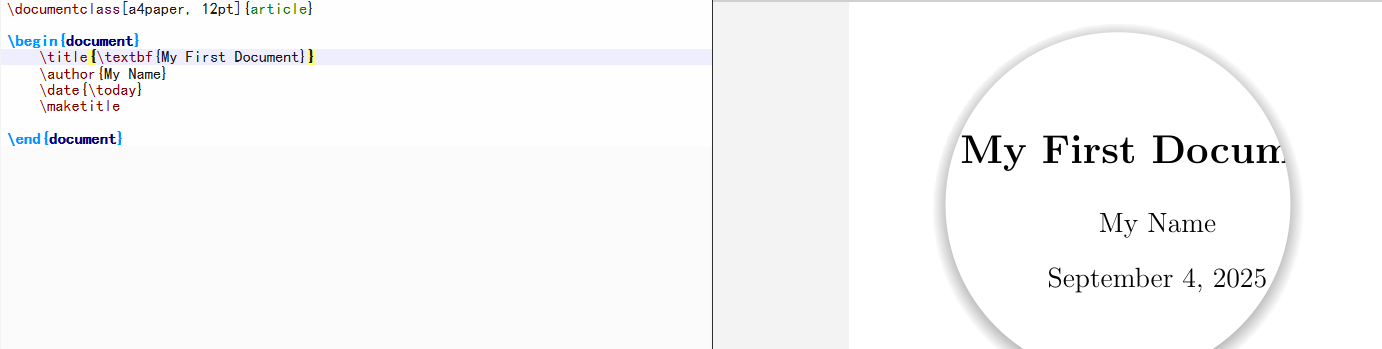
\includegraphics[width=1\textwidth]{i.png}
		\caption{实例6:textbf设置粗体}
		\label{fig:example8}
	\end{figure}
	
	\newpage
	
	7.使用graphicx包做图片相关处理。见图\ref{fig:example9}
	
	\begin{figure}[h]  
		\centering
		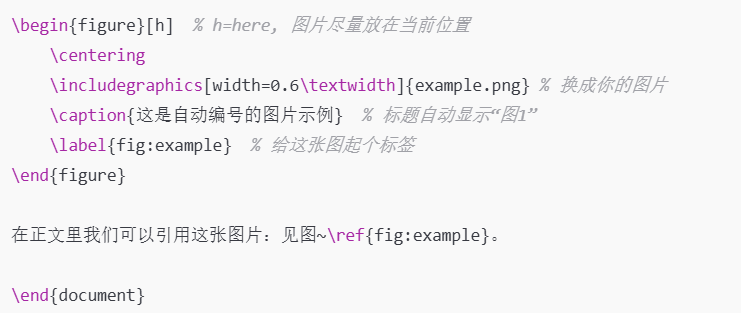
\includegraphics[width=1\textwidth]{j.png}
		\caption{实例7:graphicx插入}
		\label{fig:example9}
	\end{figure}
	
	8.使用ctex和xeletax识别中文。见图\ref{fig:example10}
	
	\begin{figure}[h]  
		\centering
		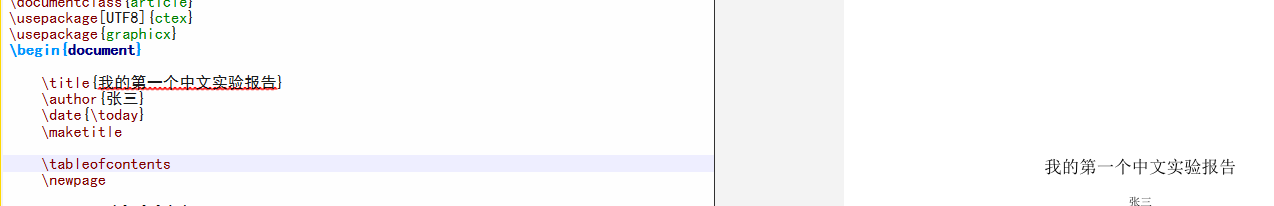
\includegraphics[width=1\textwidth]{k.png}
		\caption{实例8:中文处理}
		\label{fig:example10}
	\end{figure}
	
	9.使用tikz和eso-pic调整背景。见图\ref{fig:example11}

		\begin{figure}[h]  
		\centering
		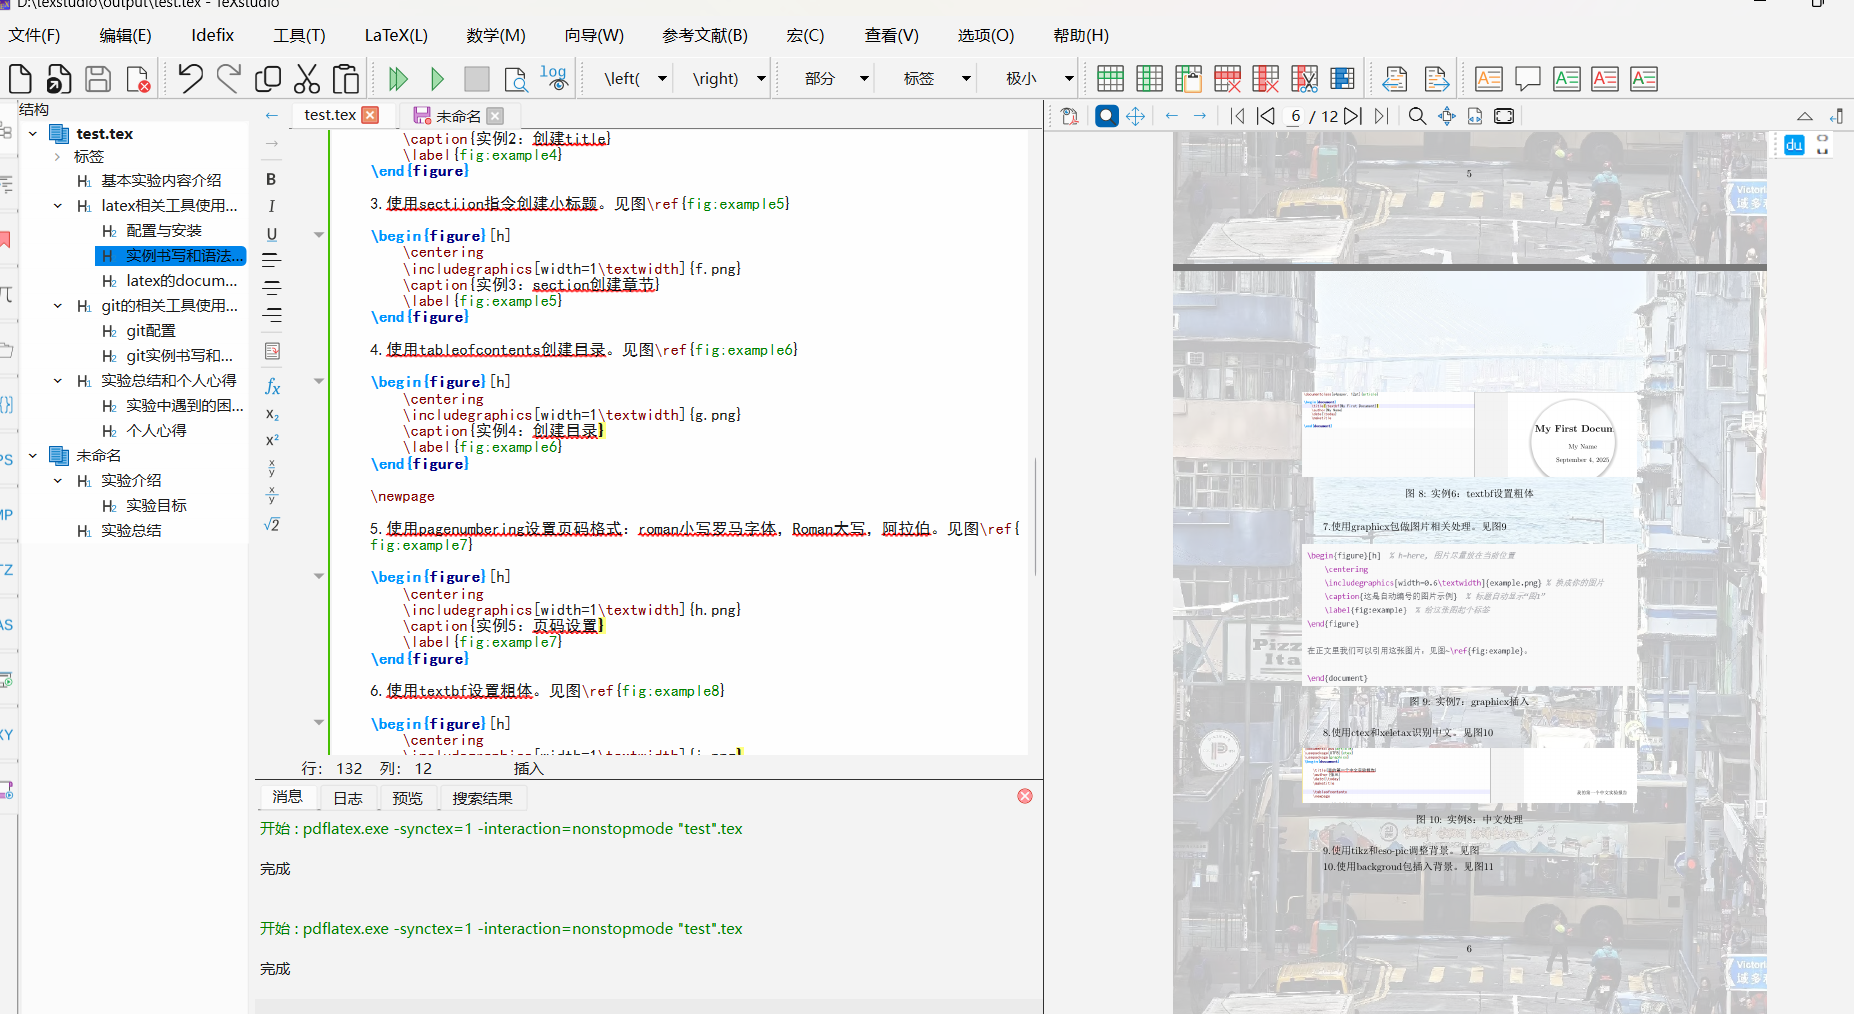
\includegraphics[width=1\textwidth]{l.png}
		\caption{实例9,tikz,eso-pic解决pdf坐标系问题}
		\label{fig:example11}
	\end{figure}
	
	\newpage
	
	10.使用backgroud包插入背景。见图\ref{fig:example12}
	
		\begin{figure}[h]  
		\centering
		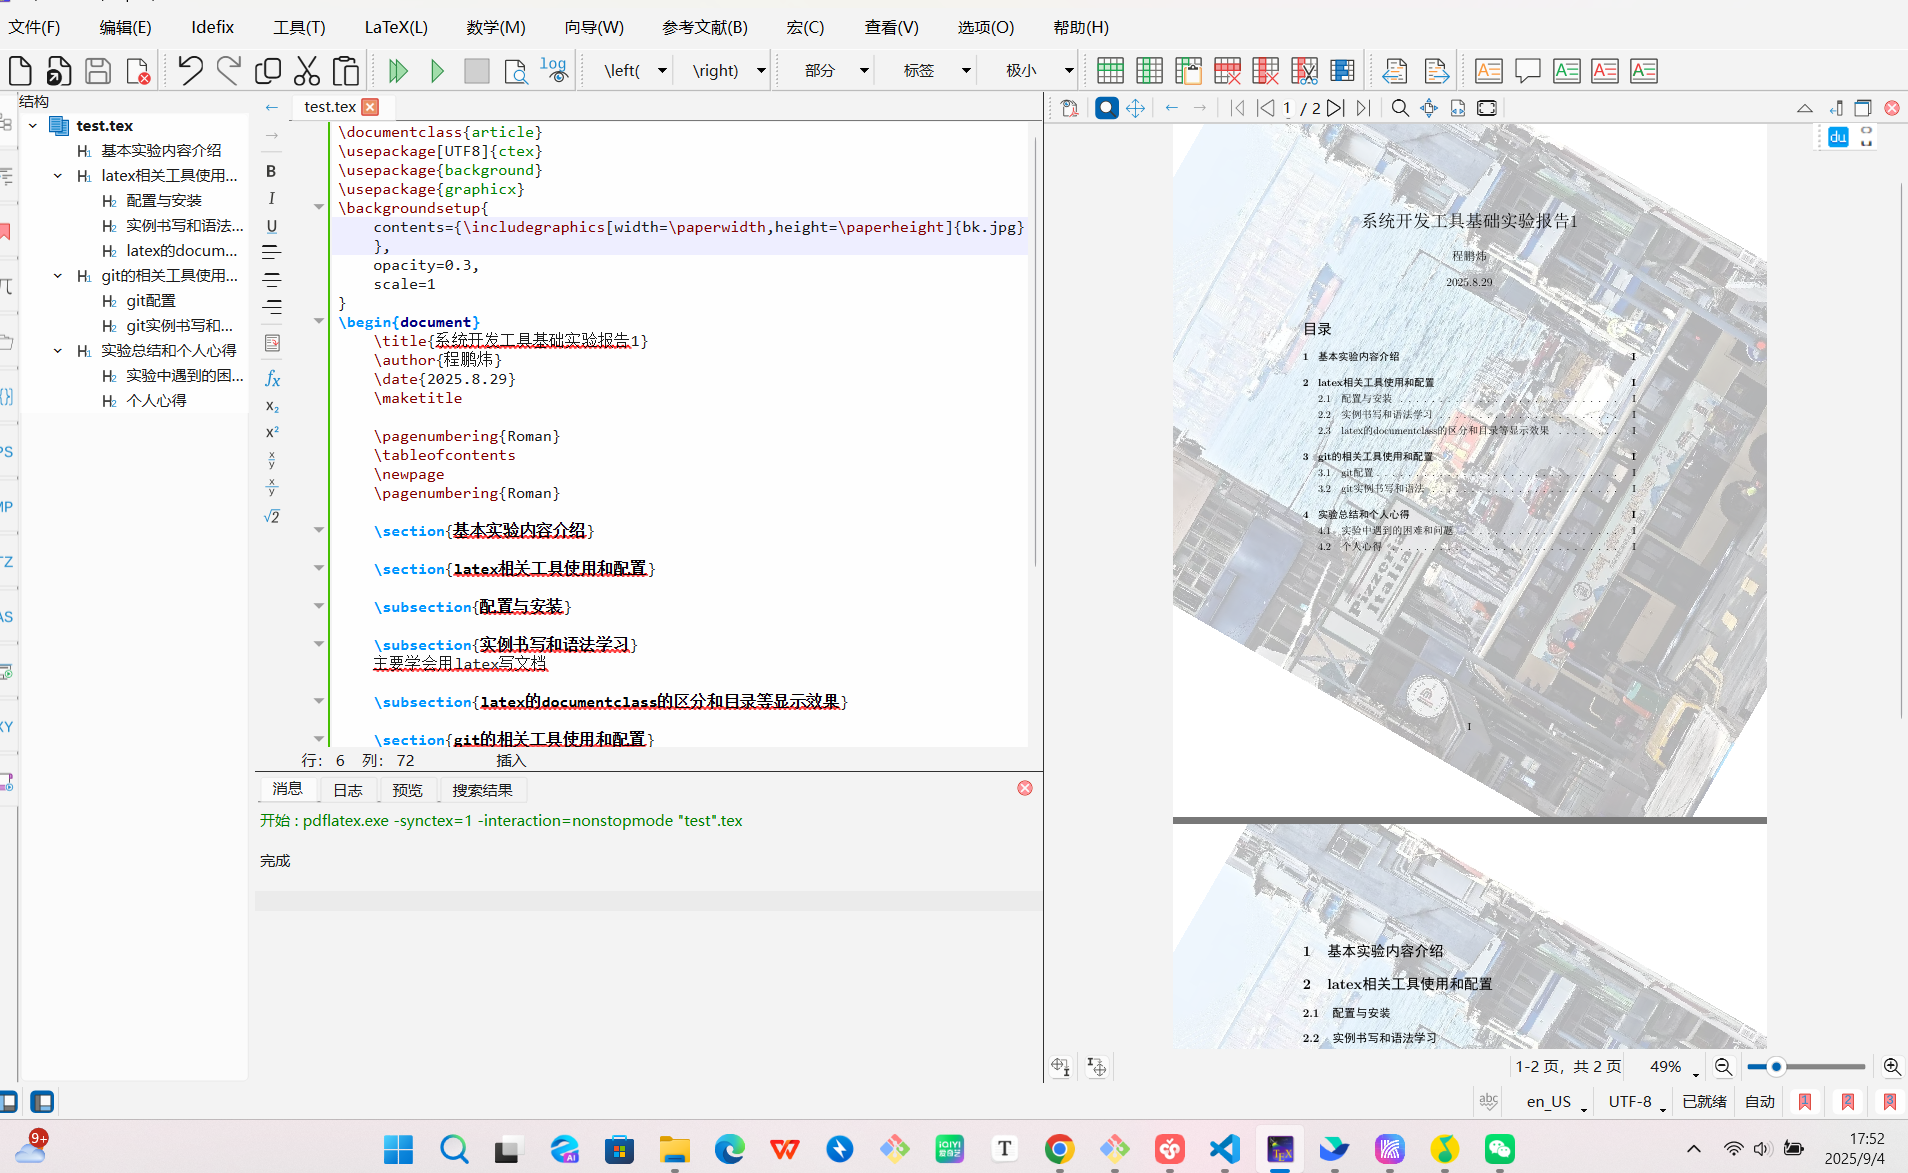
\includegraphics[width=1\textwidth]{c.png}
		\caption{实例10:backgroud指令}
		\label{fig:example12}
	\end{figure}
	
	\newpage
	
	\subsection{latex的documentclass的区分和目录等显示效果}
	这里做一个简单的介绍,算是实验中遇到的问题,由于documentclass的不同导致很多相同指令的输出效果是不一样的,最明显的就是目录的显示效果,和一些特殊指令的使用,比如report的目录显示所有的都带个0,好像是和chapter指令有关,因为我创建的是section所以0个chapter看起来很丑,所以我还是改成了article类。
	\newpage
	\section{git的相关工具使用和配置}
	\subsection{git配置}
	git配置由于下载git和mingw比较久远,本次实验并未重新配置。不再介绍。
	git
	\subsection{git实例书写和语法}
	主要是上传github和实例书写
	
	实例列举:
	
	1.设置git的用户和邮箱,见图\ref{fig:example13}
		\begin{figure}[h]  
		\centering
		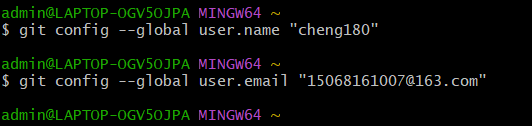
\includegraphics[width=1\textwidth]{1.png}
		\caption{实例1:设置}
		\label{fig:example13}
	\end{figure}
	
	2.对应文件夹下创建git仓库,见图\ref{fig:example14}
	
	\newpage
	\section{实验总结和个人心得}
	\subsection{实验中遇到的困难和问题}
	主要是安装latex相关编译器和ide的时候遇到的问题
	\newpage
	\subsection{个人心得}
	
\end{document}
